\documentclass[10pt,english]{beamer}
%\documentclass[english,handout]{beamer} % For handouts
\usetheme[progressbar=frametitle,block=fill]{metropolis} %numbering=none

%%% USEFUL PACKAGES
%\usepackage{showframe} % For debugging positioning
\usepackage{etex} % If too many packages
% Encoding and language
\usepackage[utf8]{inputenc}
\usepackage{babel}
\usepackage{amsmath, amssymb}
\usepackage{natbib}
%\usepackage{booktabs}
%\usepackage{algorithmic}
\usepackage{algorithm}
\usepackage{caption}
%\usepackage{animate} % Animations
\usepackage{bm} % Bold math
\usepackage{bbm}
%\usepackage{url}
%\usepackage{pifont}
%\usepackage{ulem} % Used for strikeouts \sout
%\usepackage{stackengine}
%\usepackage{enumitem}
%\setlist[description]{leftmargin=\parindent,labelindent=\parindent}
%\usepackage{colortbl} % Used for colored rows in tables


%%% GRAPHICS
\usepackage{graphicx}
\graphicspath{{./figs/}}


%%% COLORS
\setbeamercolor{background canvas}{bg=white}
\def\BlankFrame{
	\bgroup
	%\pdfpageheight 29.7cm
	\setbeamercolor{background canvas}{bg=}
	\begin{frame}[plain]
	\end{frame}
	%\makeatletter
	%\pdfpageheight \beamer@paperheight
	%\makeatother
	\egroup}

\usepackage{xcolor}
\definecolor{DarkGreen}{HTML}{00B200}
\definecolor{LightBlue}{HTML}{0090D9}
\definecolor{gold}{rgb}{.812,.710,.231}
% Text markup
%\setbeamercolor{alerted text}{fg=red}
\newcommand{\blue}[1]{\textcolor{blue}{#1}}
\newcommand{\red}[1]{\textcolor{red}{#1}}
\newcommand{\grey}[1]{\textcolor{gray}{#1}}
\newcommand{\orange}[1]{\textcolor{mLightBrown}{#1}}
\newcommand\myheading[1]{\textbf{#1}}
\newcommand\myemph[1]{\underline{\emph{#1}}}
\newcommand\textexample[1]{\textit{\textbf{#1}}}

%%% SPACING
\newcommand\vws[1][1]{\vspace{#1\baselineskip}} % vertical white space
%\newcommand\strt[1][1.5ex]{\rule[-.05\baselineskip]{0pt}{#1}} % strut
\newcommand\strt[2]{\rule[-#1ex]{0pt}{#2ex}} % strut
\newcommand\Hrule{\vspace{1ex} \hrule \vspace{1ex}} % Horisontal rule with some space after

%%% MISC
\newcommand\articleref[4]{\noindent\begin{minipage}[t]{0.04\textwidth}
		\vspace{0pt} 
		\pgfuseimage{beamericonarticle}
	\end{minipage}%
	\begin{minipage}[t]{0.96\textwidth}
		\vspace{0pt}
		#1. \textbf{#2.} \textit{#3}, #4.
	\end{minipage}}

%%% METROPOLIS THEME SPECIFIC
\makeatletter
\setlength{\metropolis@progressonsectionpage@linewidth}{1pt}
\makeatother
%\setbeamercolor{progress bar}{fg=red,bg=red!50}


%%% TEXTPOS
\usepackage[absolute,overlay]{textpos} % option showboxes is useful in draft mode
\setlength{\TPHorizModule}{\paperwidth}
\setlength{\TPVertModule}{\paperheight}
\textblockorigin{0pt}{10mm} % start everything at top-left, below gray 


%%% TIKZ/PGFPLOTS
\usepackage{tikz}
\usetikzlibrary{arrows,positioning,calc,shapes.geometric}
%\usetikzlibrary{arrows,calc,shapes.geometric,decorations.pathmorphing,backgrounds,positioning,fit,petri,decorations.pathreplacing}
%\usepackage{pgfplots}
%\pgfplotsset{compat = 1.3}


%%% BLOCKS AND BOXES
% Changing colors of blocks
%\setbeamercolor{block title alerted}{bg=UURed,fg=palette primary.fg}
%\setbeamercolor{block body alerted}{bg=UURed!15}
\setbeamercolor{block title alerted}{bg=mLightBrown,fg=palette primary.fg}
\setbeamercolor{block body alerted}{bg=mLightBrown!15}
%\setbeamercolor{block title example}{bg=UUGreen,fg=palette primary.fg}
%\setbeamercolor{block body example}{bg=UUGreen!10}
% \mybox is a rectangular box
\usepackage{boxedminipage}
\setlength\fboxrule{2pt}
\setlength\fboxsep{2\fboxsep}
\newcommand\mybox[3][\textwidth]{
  {\color{#2}
    \begin{boxedminipage}{#1}
      {\color{palette primary.bg} #3}
    \end{boxedminipage}}%
}   
\usepackage{tcolorbox}
\tcbset{arc=1mm,grow to left by=3mm,grow to right by=3mm,left=2mm}
%\newenvironment{redbox}{%
%	\begin{tcolorbox}[colback=UURed!15,colframe=UURed]}{%
%	\end{tcolorbox}}
%\newenvironment{greenbox}{%
%	\begin{tcolorbox}[colback=UUGreen!15,colframe=UUGreen]}{%
%	\end{tcolorbox}}
\newenvironment{redbox}{%
	\begin{tcolorbox}[colback=red!15,colframe=red]}{%
	\end{tcolorbox}}
\newenvironment{greenbox}{%
	\begin{tcolorbox}[colback=DarkGreen!15,colframe=DarkGreen]}{%
	\end{tcolorbox}}
\newenvironment{graybox}{%
	\begin{tcolorbox}[colback=mDarkTeal!5,colframe=mDarkTeal]}{%
	\end{tcolorbox}}
\newenvironment{orangebox}{%
\begin{tcolorbox}[colback=mLightBrown!15,colframe=mLightBrown]}{%
	\end{tcolorbox}}
\newenvironment{bwbox}{%
	\begin{tcolorbox}[colback=white,colframe=black]}{%
\end{tcolorbox}}
\newenvironment{bluebox}{%
	\begin{tcolorbox}[colback=LightBlue!15,colframe=LightBlue]}{%
\end{tcolorbox}}


%%%%%%%%% NEW MACROS

\newcommand\imp[1]{\alert{\textbf{#1}}}
\newcommand\bfit[1]{\textbf{\textit{#1}}}
\newcommand\good{\color{DarkGreen}{$\blacktriangle$}} % used in lists
\newcommand\bad{\color{red}{$\blacktriangledown$}} % used in lists


\RequirePackage{amsmath, amssymb}
\RequirePackage{bbm}
%\RequirePackage{newtxmath}


% Convenience macro for referring to data source
\newcommand\sourceurl[2]{\small \grey{Data from \href{#1}{#2}}}

% Abbreviations
\RequirePackage{xspace}
\newcommand\pdf{pdf\xspace}
\newcommand\ifft{iff\xspace}
\newcommand\ex{\textbf{ex)}\xspace}

% General time series notation
\newcommand\T{n}  % Length of time series
\newcommand\rtheta{{\red{\theta}}}  % Parameter (color coded)
\newcommand\rthetah{{\red{\widehat\theta}}}  % Estimate (color coded)

% Neural netowkrs
\newcommand\h{\mathbf{h}} % Hidden state variable
\newcommand\zz{\mathbf{z}} % Generic input (vector)

% For OLS/AR
\newcommand\noise{\varepsilon}  % This is the noise in AR, but should it be the same as measurement noise in SSM?
\newcommand\noisevar{\sigma^2_\noise}
\newcommand\noisevarhat{\widehat\sigma^2_\noise}
\newcommand\X{\Phi}
\newcommand\y{\mathbf{y}}
\newcommand\bphi{\bm\phi}

% State space models
\newcommand\z{\alpha}  % State vector, general SSM
\newcommand{\obsnoise}{\varepsilon}
\newcommand{\statenoise}{\eta}
\newcommand{\varobs}{\sigma^2_{\varepsilon}}
\newcommand{\varstate}{\sigma^2_{\eta}}
% For structural time series
\newcommand{\trendnoise}{\zeta}
\newcommand{\seasnoise}{\omega}
\newcommand{\vartrend}{\sigma^2_{\trendnoise}}
\newcommand{\varseas}{\sigma^2_{\seasnoise}}

%
\newcommand\FF{T}
\newcommand\GG{R}
\newcommand\HH{Z}
\newcommand{\covobs}{\sigma_\epsilon^2}
\newcommand{\covstate}{Q}
\newcommand\initmean{a_1}
\newcommand\initcov{P_1}
% Kalman filter
\newcommand{\zpart}[2]{\z_{#1}^{#2}}
\newcommand{\wgt}[2]{\omega_{#1}^{#2}}
\newcommand{\wgtsum}[1]{\Omega_{#1}}
\newcommand\zhat[2]{\hat\z_{#1|#2}}
\newcommand\Phat[2]{P_{#1|#2}}
\newcommand\zpred[1]{\zhat{#1}{#1-1}}
\newcommand\Ppred[1]{\Phat{#1}{#1-1}}
\newcommand\zfilt[1]{\zhat{#1}{#1}}
\newcommand\Pfilt[1]{\Phat{#1}{#1}}
\newcommand\ypred[1]{\hat y_{#1|#1-1}}
\newcommand\Spred[1]{F_{#1|#1-1}}
\newcommand\Spredinv[1]{\Spred{#1}^{-1}}
\newcommand\epshat[2]{\hat{\obsnoise}_{#1|#2}}
\newcommand\etahat[2]{\hat{\statenoise}_{#1|#2}}

\newcommand{\statefun}{T}
\newcommand{\obsfun}{Z}
\newcommand{\estfun}{h}

\newcommand{\qd}{q} %State density
\newcommand{\md}{g} %Measure density

\newcommand{\rmd}{\mathrm{d}}

% SMC
\newcommand{\Np}{N}           % Number of particles
\newcommand{\Mp}{M}           % Number of particles in backward simulation



%\RequirePackage{color}
%\newcommand{\flnote}[1]{{\color{red}\textbf{[#1]}}} % Used for notes in text - color red
%\newcommand\Hrule{\vspace{1ex} \hrule \vspace{1ex}} % Horisontal rule with some space after; This is moved to beamer preamble

%%%%%%%%%%%%%%%%%%%%%%%%%%%%%%%%%%%%%%%%%%%%%%%%%%%%%%%%%%%%%%%%%%%%%%%%%%%%%%%%
%                            COMMANDS IN TEXT                                  %
%%%%%%%%%%%%%%%%%%%%%%%%%%%%%%%%%%%%%%%%%%%%%%%%%%%%%%%%%%%%%%%%%%%%%%%%%%%%%%%%
\newcommand\numtext[2]{#1\textsuperscript{#2}}
\newcommand\thsnd[1]{\ensuremath{#1\thinspace000}}
\newcommand{\peqref}[1]{\eqref{#1} on page~\pageref{#1}} % Page referencing for equations: "(1) on page 1"

%%%%%%%%%%%%%%%%%%%%%%%%%%%%%%%%%%%%%%%%%%%%%%%%%%%%%%%%%%%%%%%%%%%%%%%%%%%%%%%%
%                            SPECIFIC MATH                                     %
%%%%%%%%%%%%%%%%%%%%%%%%%%%%%%%%%%%%%%%%%%%%%%%%%%%%%%%%%%%%%%%%%%%%%%%%%%%%%%%%
% Models etc.
%\newcommand{\T}{T}            % Number of samples in data record
\newcommand{\parspace}{\Theta}                                   % Parameter space
\newcommand{\parameter}{\theta}                                  % Parameter
% Spaces
\newcommand{\setX}{\ensuremath{\mathsf{X}}}                      % State-space X
\newcommand{\sigmaX}{\ensuremath{\mathcal{X}}}                   % Sigma algebra on X
\newcommand{\setY}{\ensuremath{\mathsf{Y}}}                      % State-space Y
\newcommand{\sigmaY}{\ensuremath{\mathcal{Y}}}                   % Sigma algebra on Y
\newcommand{\setZ}{\ensuremath{\mathsf{Z}}}                      % State-space Z
\newcommand{\sigmaZ}{\ensuremath{\mathcal{Z}}}                   % Sigma algebra on Z

%%%%%%%%%%%%%%%%%%%%%%%%%%%%%%%%%%%%%%%%%%%%%%%%%%%%%%%%%%%%%%%%%%%%%%%%%%%%%%%%
%                           GENERAL MATH                                       %
%%%%%%%%%%%%%%%%%%%%%%%%%%%%%%%%%%%%%%%%%%%%%%%%%%%%%%%%%%%%%%%%%%%%%%%%%%%%%%%%

% ======== Miscellaneous symbols ========
\newcommand\eqdef{:=}
\newcommand\defeq{=:}
\newcommand\const{\text{const.}}
%\newcommand\eqdef{\stackrel{\text{\scriptsize def}}{=}}

\newcommand\iid{iid}
\newcommand{\iidsim}{\stackrel{\text{\iid}}{\sim}} % iid simulation
\newcommand{\process}[1]{\{#1\}_{t\geq 1}}       % Process (time index t)
\newcommand{\range}[2]{#1, \, \dots, \, #2}      % Range = 1, ..., N
\newcommand{\crange}[2]{\{#1, \, \dots, \, #2\}} % Curly range = {1, ..., N}
\newcommand{\prange}[2]{(#1, \, \dots, \, #2)}   % Parenthesised range = (1, ..., N)
\newcommand{\bwdrange}[2]{#1 : -1 : #2}          % Range = N, ..., 1
\newcommand{\approxpropto}{\stackrel{\sim}\propto}

% Tight dots between \int and \int in a multidimensional integral
\newcommand{\tightcdots}{\hspace*{-0.38em}\cdot\hspace*{-0.3em}\cdot\hspace*{-0.3em}\cdot\hspace*{-0.38em}}

% Arrows - convergence and mappings
% \mapsto                                                     % Mappings, x \mapsto f(x)
\newcommand{\fromto}{\rightarrow}                             % Mapping from set A to set B; f: A \fromto B
\newcommand{\goesto}{\rightarrow}                             % limits used in n \goesto \infty
\newcommand{\goestosmall}{\to}                                % limits used in \lim_{n \goestosmall \infty}
\newcommand{\convP}{\stackrel{\probab}\longrightarrow}        % Convergence in probability
\newcommand{\convD}{\stackrel{\textrm{D}}\longrightarrow}     % Convergence in distribution

% ======== Standard spaces  ========
\newcommand{\naturals}{\ensuremath{\mathbb{N}}}               % Natural numbers
\newcommand{\reals}{\ensuremath{\mathbb{R}}}                  % Real numbers
\newcommand{\nonnegatives}{\reals_{\smaller +}}               % Nonnegative numbers
\newcommand{\positives}{\reals_{\smaller ++}}                 % Positive numbers
\newcommand{\nonnegativedefinites}[1]{S_{\smaller +}(#1)}     % Nonnegative #1 x #1 matrices
\newcommand{\positivedefinites}[1]{S_{++}(#1)}                % Positive #1 x #1 matrices

% ======== Matrices ========
\newcommand{\eye}[1]{I_{#1}}                     % Identity matrix
\newcommand{\+}{\mathsf{T}}                      % Transpose
\newcommand{\kronecker}{\raisebox{1pt}{\ensuremath{\otimes}}} % Kronecker product
\DeclareMathOperator*\diag{diag}
\DeclareMathOperator*\trace{tr}

% ======== Operators, calculus etc. ========
\newcommand{\Ordo}{O}                            % Big ordo
\newcommand{\supnorm}[1]{\|#1\|_\infty}          % Supremum norm
\newcommand\osc{\text{osc}}                      % Oscillator norm
\newcommand{\grad}{\nabla}                       % Gradient
\newcommand{\complementof}[1]{\ensuremath{#1^\mathsf{c}}} % Set complement
\renewcommand\vec{\text{vec}}
\DeclareMathOperator*\supp{supp}                          % Support
\DeclareMathOperator*\card{card}                          % Set cardinality
\DeclareMathOperator*\rank{rank}                          % Rank
\DeclareMathOperator*\sign{sign}                          % Signum function
\DeclareMathOperator*\argmax{arg\,max}
\DeclareMathOperator*\argmin{arg\,min}

% ======== Probability ========
\newcommand{\Prb}{\ensuremath{\mathbb{P}}}                       % Probability
\newcommand{\E}{\ensuremath{\mathbb{E}}}                         % Expectation
\newcommand{\var}{\ensuremath{\mathrm{Var}}}                     % Variance
\newcommand{\cov}{\ensuremath{\mathrm{Cov}}}                     % Covariance
\newcommand{\cor}{\ensuremath{\mathrm{Corr}}}                     % Correlation
\newcommand{\I}{\ensuremath{\mathbbm{1}}}						 % Indicator function

%\newcommand{\abscont}{\ensuremath{\ll}}          % Absolute continuity
\renewcommand\mid{\,\vert\,} % I don't really like that \mid produces rubber lengths. Sometimes, we get very large white spaces p(x    |   y), and it can produce line breaks after "p(x |" . Is the non-rubber definition here better?
\newcommand\Mid{\,\middle\vert\,} % Stretchable |, to use with \left \right - N.B. This produces a longer | in general. Does that look better than a standard \mid?


% Distributions
\newcommand{\N}{\ensuremath{\mathcal{N}}}        % Normal
\newcommand{\uni}{\ensuremath{\mathcal{U}}}      % Uniform
\newcommand\MN{\mathcal{MN}}                     % Matrix normal
\newcommand\IW{\mathcal{IW}}                     % Inverse-Wishart
\newcommand\GP{\mathcal{GP}}                     % Gaussian process
\DeclareMathOperator*\Mult{Mult}                 % Multinomial
\DeclareMathOperator*\cat{Cat}                   % Categorical
\DeclareMathOperator*\Discrete{Discrete}         % Categorical/alternative name
\DeclareMathOperator*\bin{Bin}                   % Binomial
\DeclareMathOperator*\gam{Gam}                   % Gamma
\DeclareMathOperator*\St{St}                     % Student's t
\DeclareMathOperator*\po{Po}                   % Binomial

%\usepackage{extendedalt}
%\usepackage{animate} % Animations
%\usepackage{../lindsten}
%\usepackage{movie15}
\usepackage{tikz}
\usepackage{listofitems} % for \readlist to create arrays

\title{732G12 Data Mining}
\subtitle{Föreläsning 10}
\date{}
\author{Johan Alenlöv \\ IDA, Linköping University, Sweden}
\titlegraphic{\hfill
\includegraphics[height=1.2cm]{../LiU_primary_black.pdf}}
%\institute{Joint work with\dots}


%% MY DEF %%
\newcommand{\itm}[1]{\mathrm{Item}_{#1}}
\newcommand{\pausa}{\pause}
%\renewcommand{\pausa}{}
\tikzstyle{mynode}=[thick,draw=blue,fill=blue!20,circle,minimum size=22]


\newenvironment{nscenter}
 {\parskip=0pt\par\nopagebreak\centering}
 {\par\noindent\ignorespacesafterend}

\begin{document}

\maketitle

\begin{frame}{Dagens föreläsning}

    \begin{itemize}
        \item One-Dimensional Kernel Smoothers
        \item Lokal Regression
        \item Generaliserade Additativa Modeller
        \item Sammanfattning av Kursen
    \end{itemize}
    
\end{frame}

\begin{frame}{One-Dimensional Kernel Smoothers}

    Vi tänker oss tillbaka till KNN och dess användning vid regression.
    \begin{equation*}
        \hat{g}(x) = \operatorname{Medel}(y_i | x_i \in N_k(x)).
    \end{equation*}

    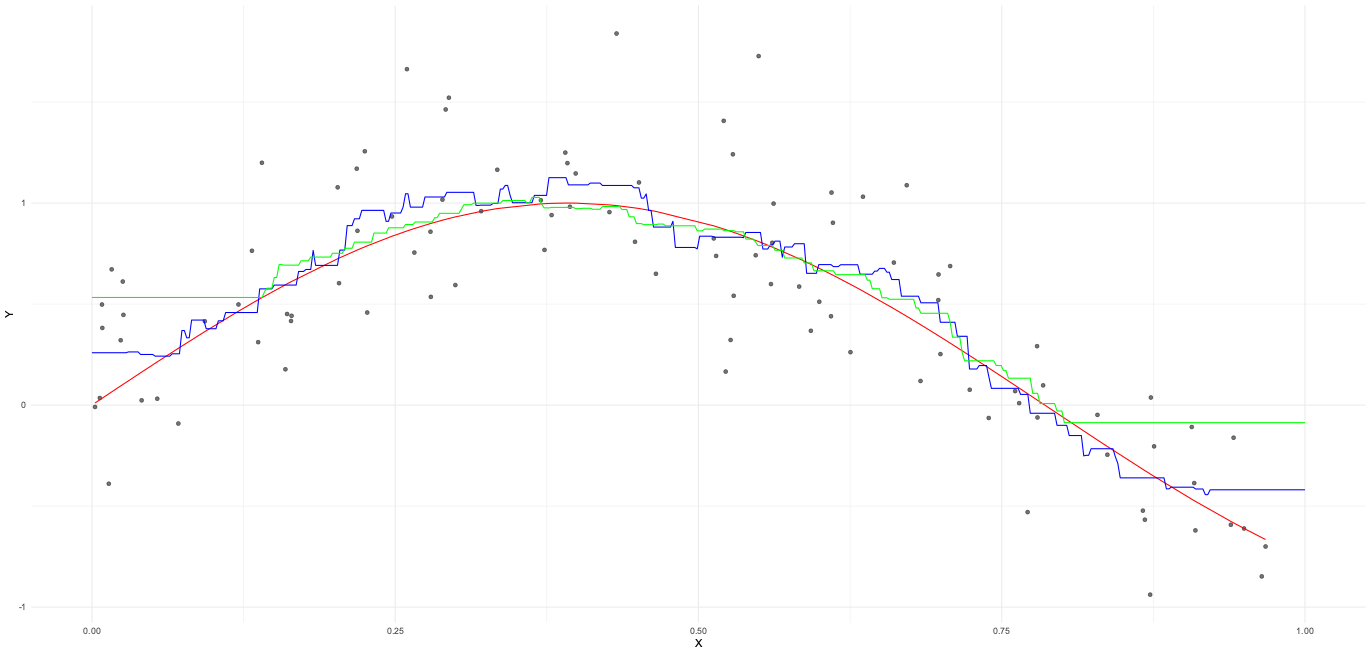
\includegraphics[width=\textwidth]{fig/knnreg.png}

    Blå har $K=10$ och grön $K=30$.
\end{frame}

\begin{frame}{One-Dimensional Kernel Smoothers}

    \begin{itemize}
        \item Problem med hopp i funktionen.
        \item Ett sätt att lösa det är att vikta om punkterna.
    \end{itemize}

    Vi vill estimera $g(x_0)$ men istället för att ge alla närliggande punkterna samma vikt så använder vi
    \begin{equation*}
        \hat{g}(x_0) = \frac{\sum_{i=1}^{n} K_{\lambda}(x_0, x_i) y_i}{\sum_{i=1}^{n}K_{\lambda}(x_0, x_i)},
    \end{equation*}
    där $K_{\lambda}(x_0, x_i)$ är en viktfunktion (Kernel).
\end{frame}

\begin{frame}{One-Dimensional Kernel Smoothers}
    
    Kernel-funktionen är en täthet, vanligtvis given på formen
    \begin{align*}
        K_{\lambda} (x_0, x_i) &= D\left(\frac{|x_0 - x_i|}{\lambda}\right) \\
        D(t) &\propto \begin{cases}
            (1 - |t|^p)^q,& \quad \text{om } |t| \leq 1, \\
            0& \text{annars.}
        \end{cases}
    \end{align*}
    eller $D(t)$ är täthetsfunktionen för en standard normalfördelning. $\lambda$ kallas för "bandwidth".

    \begin{description}
        \item[Triangel] : $p = 1, q = 1$
        \item[Epanechnikov] : $p = 2, q = 1$
        \item[Quartic] : $p = 2, q = 2$ 
        \item[Tri-cube] : $p = 3, q = 3$  
    \end{description}
    

\end{frame}

\begin{frame}{One-Dimensional Kernel Smoothers}

    Vi testar tre olika kernels (Triangel - Grön, Epanechnikov - Brun, Quartic - Blå) och får följande resultat

    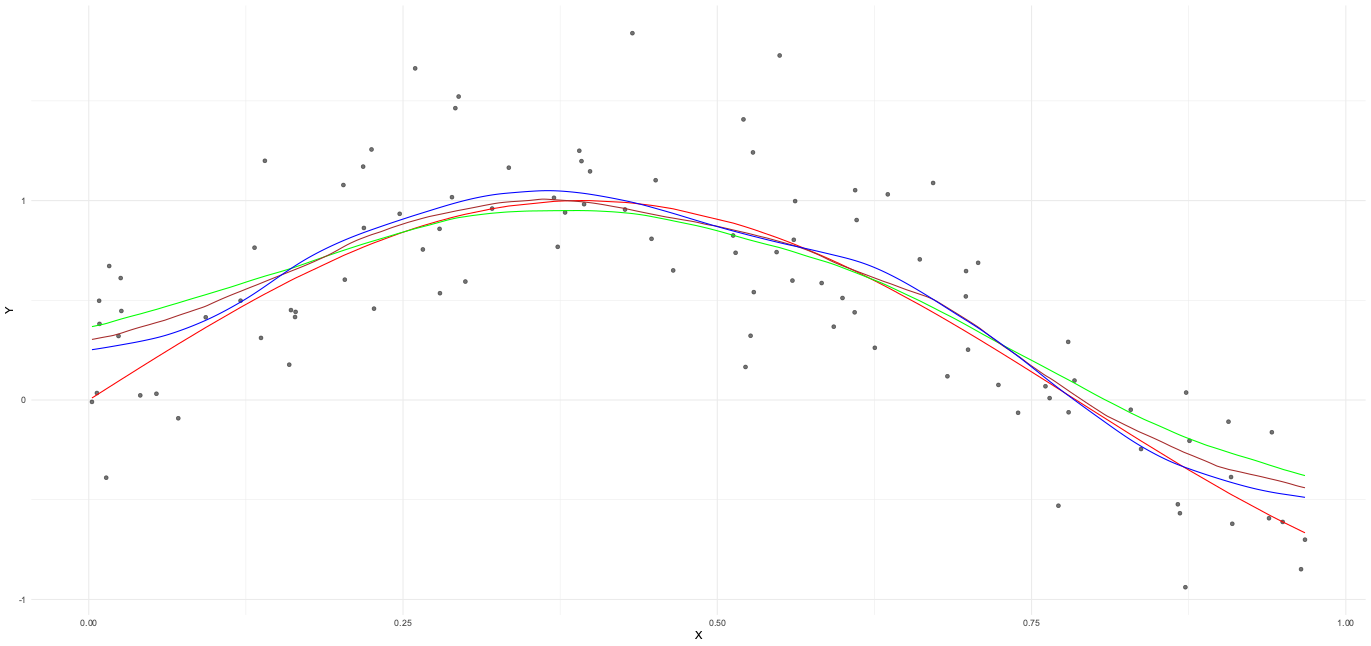
\includegraphics[width = \textwidth]{fig/kernel.png}
    
\end{frame}

\begin{frame}{One-Dimensional Kernel Smoothers}

    \begin{itemize}
        \item Ett sätt att göra "viktat KNN" som ger en "mjuk" funktion.
        \item Vanligtvis sätter vi inte ett antal grannar.
        \begin{itemize}
            \item Låter $\lambda$ styra hur stort fönster vi kollar i.
        \end{itemize}
        \item Många olika val av kernels.
        \item Problem vid kanterna.
    \end{itemize}
    
\end{frame}

\begin{frame}{Lokal Regression}

    Vi har sedan tidigare delat upp variabelrummet i olika delar och gjort regression på varje del.

    Istället för att dela upp rummet i förväg och göra regression i varje del, varför inte välja ett intervall runt den punkt där vi vill beräkna regressionen?

    Hur välja område?
    
\end{frame}

\begin{frame}{Lokal Regression}
    Inspirerat av det One-Dimensio Kenel Smoothers
    \begin{greenbox}
        Gör (linjär) regression vid en punkt $x_0$ där vi viktar alla fel med en kernel.
    \end{greenbox}

    För varje punkt $x_0$ där vi vill beräkna funktionen löser vi ett regressionsproblem
    \begin{equation*}
        \min_{\mathbf{\beta}(x_0)} \sum_{i=1}^{n} K_{\lambda}(x_0, x_i) [y_i - \beta_0(x_0) + \beta_1(x_0) x_i]^2.
    \end{equation*}

\end{frame}

\begin{frame}{Lokal Regression}
    Skattar lokal regression med olika $\lambda$ med $p = q = 3$ (Tri-Cube)

    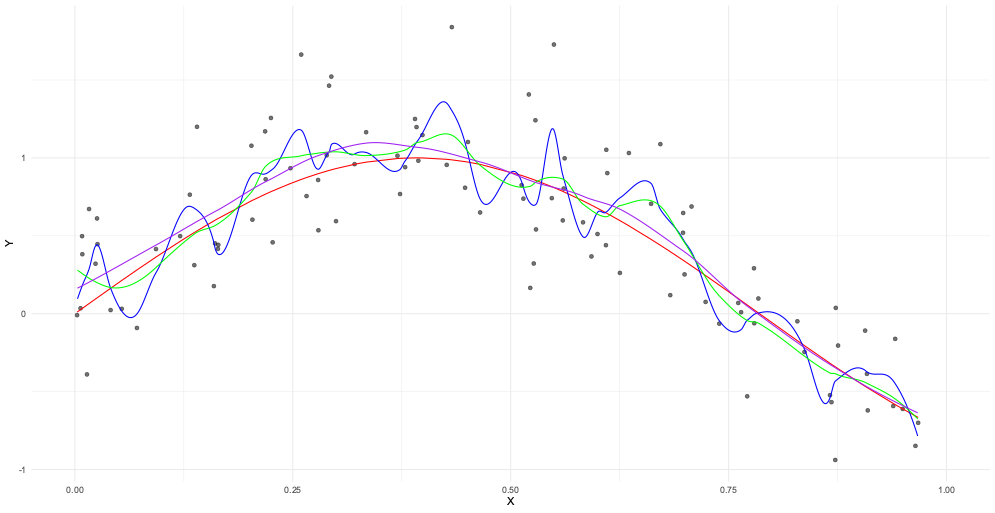
\includegraphics[width = \textwidth]{fig/locreg.png}
\end{frame}

\begin{frame}{Lokal Regression}
    
    \begin{itemize}
        \item Kan såklart göra polynomregression istället för linjär regression.
        \item Går att göra för multiple regression,
        \begin{itemize}
            \item Vanligt att man bara gör lokal regression för några enstaka parametrar.
            \item Kan göra simultan lokal regression där vi skattar ett $p$-dimensionellt plan.
            \item Funkar (generellt) dåligt för $p$ större än 4.
        \end{itemize}
    \end{itemize}

\end{frame}

\begin{frame}{Generaliserade Additativa Modeller}

    Allt det vi gjort denna och förra föreläsning handlar om att presentera flexibla modeller för att prediktera $y$ givet $x$.
    
    Nu ska vi använda detta för att skapa flexibla modeller för att prediktera $y$ givet $x_1, x_2, x_3, \ldots, x_p$.

    \begin{greenbox}
        \imp{Generaliserade Additativa Modeller} (GAM) är en generell modell för att utöka linjär regression genom att tillåta icke-linjära funktioner av varje variabel, samtidigt som modellen är additativ.
    \end{greenbox}
    
\end{frame}

\begin{frame}{Generaliserade Additativa Modeller}
    
    Gemensamt för alla GAM modeller är att vi i vår regression eller klassificerings modell byter ut
    \begin{equation*}
        \beta_0 + \beta_1 x_1 + \beta_2 x_2 + \ldots + \beta_p x_p,
    \end{equation*}
    till
    \begin{equation*}
        \beta_0 + \beta_1 g_1(x_1) + \beta_2 g_2(x_2) + \ldots + \beta_p g_p(x_p),
    \end{equation*}
    där $g_i$ är en ("mjuk") icke-linjär funktion.

\end{frame}

\begin{frame}{Generaliserade Additativa Modeller}
    
    För regression får vi följande typ av modell,
    \begin{equation*}
        y_i = \beta_0 + \beta_1 g_1(x_1) + \beta_2 g_2(x_2) + \ldots + \beta_p g_p(x_p) + \varepsilon_i,
    \end{equation*}
    där vi är fria att välja varje $g_i$ själva.

    T.ex. kan vi välja att några ska vara splines, någon kanske är en steg-funktion och någon är identitetsfunktionen.

\end{frame}

\begin{frame}{Generaliserade Additativa Modeller}
    
    För klassificering får vi följande typ av modell,
    \begin{equation*}
        \log\left(\frac{p(x)}{1 - p(x)}\right) = \beta_0 + \beta_1 g_1(x_1) + \beta_2 g_2(x_2) + \ldots + \beta_p g_p(x_p) + \varepsilon_i,
    \end{equation*}
    där vi är fria att välja varje $g_i$ själva.

    Här kan vi igen aktivt välja vilka typer av funktioner som passar bäst per variabel.

\end{frame}

\begin{frame}{Generaliserade Additativa Modeller}
    
    \begin{itemize}
        \item GAMs låter oss anpassa en icke-linjär funktion för varje förklarande variabel.
        \item Eftersom modellen är additativ kan vi fortfarande undersöka effekten av varje förklarande variabel genom att hålla de andra konstanta.
        \item Hur "mjuka" varje funktion är kan vi beskriva genom frihetsgraderna. 
        \item Den största nackdelen är att modellen måste vara additativ.
        \begin{itemize}
            \item Detta gör att interaktioner mellan variabler missas.
            \item Vi kan lägga till specifika interaktioner, men detta måste göras manuellt.
        \end{itemize}
    \end{itemize}

\end{frame}

\begin{frame}[standout]
    \Huge Sammanfattning av kursen
\end{frame}

\begin{frame}{Sammanfattning av kursen}

    Sammanfattning i en mening:
    \begin{itemize}
        \item Givet data, hitta den bästa (mest lämpade), modellen som beskriver detta dataset.
    \end{itemize}

    Till vår hjälp har vi gått igenom väldigt många olika modeller och algoritmer.
    
\end{frame}

\begin{frame}{Sammanfattning}
    \begin{itemize}
        \item Modellval
        \begin{itemize}
            \item Felfunktioner
            \item Dela upp data i träning, validering, test.
            \item Korsvalidering
            \item AIC, BIC\dots
            \item Variabelselektion
        \end{itemize}
        \item Regularisering,
        \begin{itemize}
            \item LASSO, Ridge
        \end{itemize}
    \end{itemize}
\end{frame}

\begin{frame}{Sammanfattning}
    \begin{itemize}
        \item Trädmodeller
        \begin{itemize}
            \item Dela upp variabelrummet i rektanglar.
            \item Varje rektangel får ett värde.
            \item Olika regler för uppdelning beroende på problem.
        \end{itemize}
        \item Beskärning av träd
        \begin{itemize}
            \item Förbeskärning
            \item Efterbeskärning
        \end{itemize}
        \item Ensamblemetoder
        \begin{itemize}
            \item Bagging - Använd bootstrap för att skapa många "oberoende" träd.
            \item Random forest - Gör slumpmässiga ändringar i träden.
            \item Boosting - Skapa många små träd, men modifiera datan mellan varje träd.
        \end{itemize}
    \end{itemize}
\end{frame}

\begin{frame}{Sammanfattning}
    
    \begin{itemize}
        \item K-närmaste grannar
        \begin{itemize}
            \item Skattar värdet med hjälp av närmaste datapunkterna.
            \item Kan förbättras genom att vikta med avståndet
        \end{itemize}
        \item Naive bayes
        \begin{itemize}
            \item Skatta klassificering med hjälp av bayes sats
            \item För full fördelning krävs mykcet data.
            \item Görs ofta förenklningen att varje variabel är oberoende.
        \end{itemize}
    \end{itemize}

\end{frame}

\begin{frame}{Sammanfattning}
    
    \begin{itemize}
        \item Klusteranalys
        \begin{itemize}
            \item Oövervakad inlärning.
            \item K-means klustring
            \item Hierarkisk klustring
            \item K-medoid klustring
            \item DBSCAN
        \end{itemize}
    \end{itemize}

\end{frame}

\begin{frame}{Sammanfattning}
    
    \begin{itemize}
        \item Icke-linjär regression
        \begin{itemize}
            \item Grundidé är att hitta en transformation av förklarande variabler.
            \item Gått igenom många olika transformationer.
        \end{itemize}
        \item Basfunktioner
        \item Splines
        \item Kernelfunktioner
        \item Lokal regression
        \item Neurala nätverk
        \begin{itemize}
            \item Olika typer av lager för oliak problem.
            \item Olika aktiveringsfunktioner.
            \item Global approximation theorem.
        \end{itemize}
    \end{itemize}

\end{frame}

\begin{frame}[standout]
    \Huge Tack för att ni har lyssnat!

    \large Nu är det bara projektet kvar.
\end{frame}

\end{document}